\section{The BML Traffic Model}
\label{sec:The-BML-Traffic-Model}
The \glsentryfull{bml} traffic model was first formulated in 1992 by \citet{Biham}. It consists of a variable number of cars, represented as points on a lattice that are initialized with random starting positions, where each car on said lattice belongs to either one of two classes. The first class, generally represented by cars that take on a red color, can only move towards the right on the lattice while the second class, generally represented by cars that take on a blue color, can only move downwards on the lattice. During each turn of the simulation all the cars advance by one step if and \textit{only if} they are not currently being blocked by another car \ie there exists a car  in the space directly in front of them.

\begin{figure}[htb!]
    \centering
    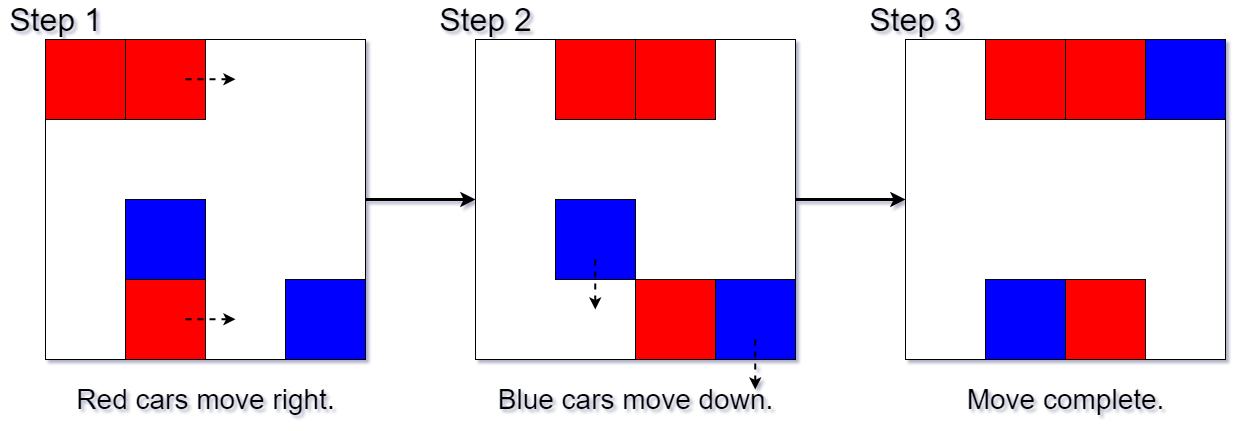
\includegraphics[width=\linewidth]{Images/Section 2/BML Step.png}
    \caption{Steps of the \gls{bml} traffic model.}
    \label{fig:BML-Step}
\end{figure}

\noindent The lattice space that the cars are placed on varies in shape with the most common shapes simulated being either a square lattice, as seen in Figure \ref{fig:BML-Torus}, or a rectangular lattice. Regardless of shape, the topology of the lattice is equivalent to a torus; that is in the sense that cars that move off the right edge would reappear on the left edge and cars that move off the bottom edge would reappear on the top edge in the case of a lattice with 4 edges.

\begin{figure}[htb!]
    \centering
    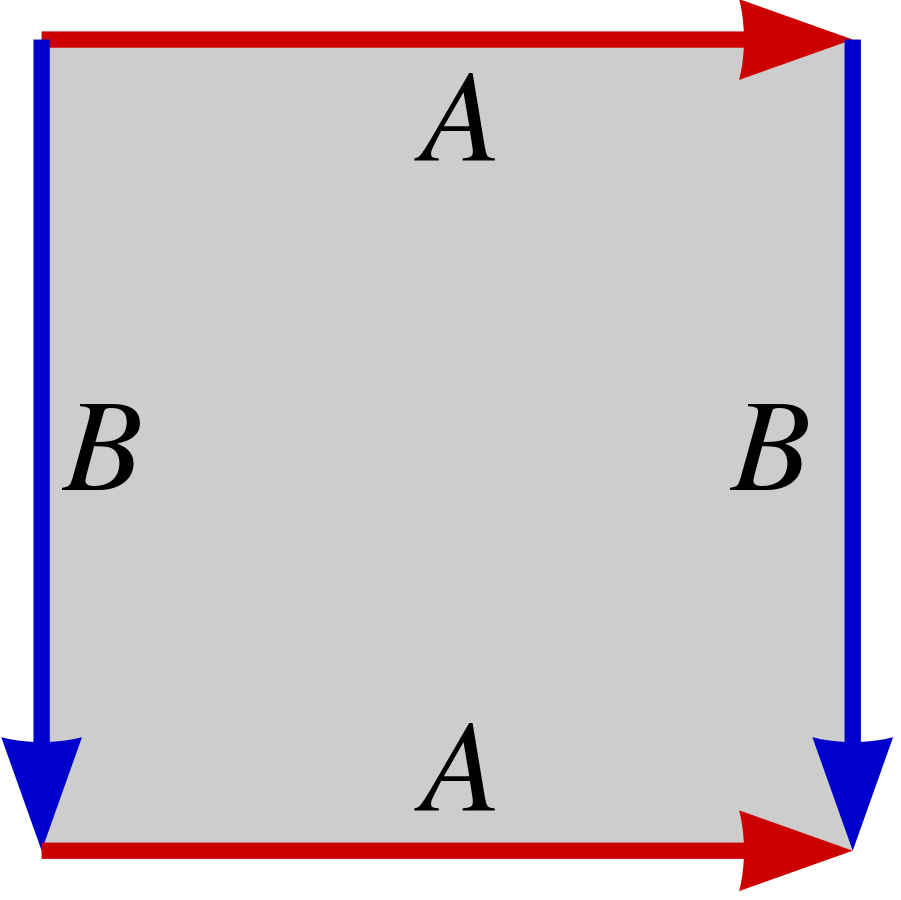
\includegraphics[width=0.25\linewidth]{Images/Section 2/BML Torus.png}
    \caption{The fundamental torus of the polygon on which the cars of both class A (\textcolor{red}{red}) and class B (\textcolor{blue}{blue}) move on. Image source: \cite{Wikipedia_Torus}, licensed under public domain.}
    \label{fig:BML-Torus}
\end{figure}

\noindent The most interesting aspects of the \gls{bml} traffic model are its two highly distinguishable phases: the jammed phased and the free-flowing phase and, as the names suggest, pertain to when the cars on the lattice organize themselves to either achieve a smooth flow of traffic or reach a globally jammed state in which not a single car can make a move. With all of that said, and in spite of the \gls{bml} traffic model's simplicity, it has been subject to rigorous mathematical analysis with \citet{Omer} noting that with densities $\rho \sim 1$ or $lim_{\rho \to 1}$ the system will reach a globally jammed phase infinitely often and \citet{Austin} noting that the model will always reach the free-flowing phase if the total number of cars $(n)$ is less than half the length of the edge of a square lattice $(\frac{N}{2})$. In this paper we will be exploring the relationship of $\rho$, or otherwise the number of the cars on the lattice, with the state of the traffic flow and attempt to recreate the findings of both \citeauthor{Omer} and \citeauthor{Austin}.